\documentclass[11pt,a4paper]{article}

% ---------------------------------------------------------------
% Tipografia: Palatino, versalete, uma cor de destaque (bordô)
% ---------------------------------------------------------------
\usepackage[utf8]{inputenc}
\usepackage[T1]{fontenc}
\usepackage[brazil]{babel}
\usepackage[sc,osf]{mathpazo}
\usepackage{microtype}
\usepackage[top=2.4cm, bottom=2.6cm, left=2.6cm, right=2.6cm]{geometry}
\usepackage{amsmath}
\usepackage{amssymb}
\usepackage{xcolor}
\usepackage{tcolorbox}
\tcbuselibrary{skins, breakable}
\usepackage{enumitem}
\usepackage{booktabs}
\usepackage{array}
\usepackage{tabularx}
\usepackage{needspace}
\usepackage{hyperref}
\usepackage{tikz}
\usepackage{pgfplots}
\usepackage{comment}
\usepackage{pdfpages}   % anexa as resolu\c{c}\~oes manuscritas no fim
\pgfplotsset{compat=1.18}
\usetikzlibrary{arrows.meta, patterns}

\definecolor{vinho}{RGB}{122, 27, 42}
\definecolor{grafite}{RGB}{70, 70, 70}
\hypersetup{colorlinks=true, linkcolor=vinho, urlcolor=vinho}

\linespread{1.06}
\setlength{\parindent}{0pt}
\setlength{\parskip}{0.45em}

% ---------------------------------------------------------------
% Formatação das questões
% ---------------------------------------------------------------
\newcommand{\selosala}{{\small\scshape\color{vinho}[fazer em sala]}\ }
\newcommand{\selobonus}{{\small\scshape\color{vinho}[sala --- b\^onus]}\ }
\newcommand{\fonte}[1]{{\small\scshape\color{grafite}#1}}

\newenvironment{questao}[2]{%
  \needspace{6\baselineskip}
  \par\addvspace{1.6em}
  {\large\bfseries\color{vinho}Quest\~ao #1}\hfill #2\\[-0.55em]
  {\color{black!25}\rule{\linewidth}{0.4pt}}
  \par\nobreak\smallskip
}{\par\addvspace{0.4em}}

\newcommand{\parte}[1]{%
  \needspace{7\baselineskip}
  \vspace{1.8em}
  {\Large\bfseries #1}\\[-0.55em]
  {\color{black!30}\rule{\linewidth}{0.5pt}}
  \par\nobreak\smallskip
}

\newtcolorbox{painel}{blanker, breakable, left=12pt,
  borderline west={1.4pt}{0pt}{black!30},
  before skip=11pt, after skip=11pt}

\setlist[enumerate,1]{label=\textbf{\alph*)}, leftmargin=2em, nosep}

% ---------------------------------------------------------------
\begin{document}
% ---------------------------------------------------------------

% ---------------------------------------------------------------
% TÍTULO
% ---------------------------------------------------------------
\thispagestyle{empty}

{\scshape\color{vinho}cursinho solid\'ario \,\textperiodcentered\, f\'isica}\\[-0.5em]
{\color{vinho}\rule{\linewidth}{1.6pt}}\\[0.9em]
{\huge\bfseries Lista de Quest\~oes}\\[0.35em]
{\LARGE Din\^amica --- Leis de Newton}\\[0.7em]
{\itshape\color{grafite}Quest\~oes reais de ENEM e de vestibulares
(UTFPR, UEL, UERJ)}
\hfill {\color{grafite}2026}\\[-0.3em]
{\color{black!30}\rule{\linewidth}{0.5pt}}

\vspace{1.0em}

\begin{painel}

\begin{itemize}[nosep, leftmargin=1.5em]
  \item Todas as quest\~oes s\~ao de provas antigas. A fonte e o ano
        est\~ao do lado do n\'umero.
  \item As quest\~oes marcadas com \selosala tem como objetivo serem resolvidas na
        aula (Bloco 5 do plano).
  \item O resto são questões extras. Come\c{c}ar por Q2, Q3 e
        Q10 (uma de cada lei); Q15 \'e o treino de diagramas de corpo
        livre com fio e roldana.
  \item Q16 e Q17 s\~ao desafios.
  \item No fim da lista tem o gabarito comentado e, depois dele, as
        \textbf{resolu\c{c}\~oes passo a passo} das quest\~oes de
        c\'alculo.
\end{itemize}
\end{painel}

\newpage

{\renewcommand{\arraystretch}{1.25}
\begin{tabular}{@{}clll@{}}
  \multicolumn{4}{@{}l}{{\scshape\color{vinho}mapa da lista}}\\
  \addlinespace[2pt]
  \toprule
  \# & Fonte & Tema & Onde \\
  \midrule
  1  & ENEM PPL 2012      & 1\textordfeminine{} Lei (in\'ercia)          & \textbf{sala} \\
  2  & ENEM PPL 2013      & 1\textordfeminine{} Lei / movimento relativo & casa \\
  3  & ENEM PPL 2014      & For\c{c}a resultante e peso                  & casa \\
  4  & UTFPR Ver\~ao 2025 & 2\textordfeminine{} Lei (num\'erica)         & \textbf{sala} \\
  5  & ENEM 2017          & 2\textordfeminine{} Lei + gr\'afico          & \textbf{sala} \\
  6  & ENEM 2009          & Massa $\times$ peso                          & casa \\
  7  & UTFPR Ver\~ao 2025 & For\c{c}a el\'astica (Lei de Hooke)          & casa \\
  8  & ENEM 2013          & 3\textordfeminine{} Lei + atrito             & \textbf{sala} \\
  9  & ENEM PPL 2012      & 3\textordfeminine{} Lei (conceito)           & \textbf{sala} \\
  10 & UTFPR Inverno 2023 & 3\textordfeminine{} Lei / propuls\~ao        & casa \\
  11 & ENEM PPL 2012      & Atrito est\'atico $\times$ cin\'etico (ABS)  & \textbf{sala} \\
  12 & UEL 1995           & Plano inclinado sem atrito                   & \textbf{sala (bonus)} \\
  13 & UERJ 1998          & Rampa: for\c{c}a m\'inima                    & casa \\
  14 & UTFPR Inverno 2024 & Blocos em contato (2\textordfeminine{} Lei)  & \textbf{sala} \\
  15 & UEL 1994           & Blocos ligados por fio + roldana             & casa \\
  16 & ENEM 2009          & Desafio: curva do trem-bala                  & casa \\
  17 & UTFPR Ver\~ao 2024 & Desafio: colis\~ao                           & casa \\
  \bottomrule
\end{tabular}}

\newpage

% ===================================================================
\parte{Parte I --- 1\textordfeminine{} Lei: In\'ercia}
% ===================================================================

\begin{questao}{1}{\selosala\fonte{ENEM PPL 2012}}
Em 1543, Nicolau Cop\'ernico publicou um livro revolucion\'ario em que
propunha a Terra girando em torno do seu pr\'oprio eixo e rodando em
torno do Sol. Isso contraria a concep\c{c}\~ao aristot\'elica, que
acredita que a Terra \'e o centro do universo. Para os aristot\'elicos,
se a Terra gira do oeste para o leste, coisas como nuvens e p\'assaros,
que n\~ao est\~ao presas \`a Terra, pareceriam estar sempre se movendo
do leste para o oeste, justamente como o Sol. Mas foi Galileu Galilei
que, em 1632, baseando-se em experi\^encias, rebateu a cr\'itica
aristot\'elica, confirmando assim o sistema de Cop\'ernico. Seu
argumento, adaptado para a nossa \'epoca, \'e: se uma pessoa, dentro de
um vag\~ao de trem em repouso, solta uma bola, ela cai junto a seus
p\'es. Mas se o vag\~ao estiver se movendo com velocidade constante, a
bola tamb\'em cai junto a seus p\'es. Isto porque a bola, enquanto cai,
continua a compartilhar do movimento do vag\~ao.

O princ\'ipio f\'isico usado por Galileu para rebater o argumento
aristot\'elico foi
\begin{enumerate}
  \item a lei da in\'ercia.
  \item a\c{c}\~ao e rea\c{c}\~ao.
  \item a segunda lei de Newton.
  \item a conserva\c{c}\~ao da energia.
  \item o princ\'ipio da equival\^encia.
\end{enumerate}
\end{questao}

\begin{questao}{2}{\fonte{ENEM PPL 2013}}
Conta-se que um curioso incidente aconteceu durante a Primeira Guerra
Mundial. Quando voava a uma altitude de dois mil metros, um piloto
franc\^es viu o que acreditava ser uma mosca parada perto de sua face.
Apanhando-a rapidamente, ficou surpreso ao verificar que se tratava de
um proj\'etil alem\~ao.
\begin{flushright}\small
PERELMAN, J. \textit{Aprenda f\'isica brincando}. S\~ao Paulo: Hemus, 1970.
\end{flushright}

O piloto consegue apanhar o proj\'etil, pois
\begin{enumerate}
  \item ele foi disparado em dire\c{c}\~ao ao avi\~ao franc\^es, freado
        pelo ar e parou justamente na frente do piloto.
  \item o avi\~ao se movia no mesmo sentido que o dele, com velocidade
        visivelmente superior.
  \item ele foi disparado para cima com velocidade constante, no
        instante em que o avi\~ao franc\^es passou.
  \item o avi\~ao se movia no sentido oposto ao dele, com velocidade de
        mesmo valor.
  \item o avi\~ao se movia no mesmo sentido que o dele, com velocidade
        de mesmo valor.
\end{enumerate}
\end{questao}

% ===================================================================
\parte{Parte II --- 2\textordfeminine{} Lei e For\c{c}as}
% ===================================================================

\begin{questao}{3}{\fonte{ENEM PPL 2014}}
Na Antiguidade, algumas pessoas acreditavam que, no lan\c{c}amento
obl\'iquo de um objeto, a resultante das for\c{c}as que atuavam sobre
ele tinha o mesmo sentido da velocidade em todos os instantes do
movimento. Isso n\~ao est\'a de acordo com as interpreta\c{c}\~oes
cient\'ificas atualmente utilizadas para explicar esse fen\^omeno.

Desprezando a resist\^encia do ar, qual \'e a dire\c{c}\~ao e o sentido
do vetor for\c{c}a resultante que atua sobre o objeto no ponto mais alto
da trajet\'oria?
\begin{enumerate}
  \item Indefinido, pois ele \'e nulo, assim como a velocidade vertical
        nesse ponto.
  \item Vertical para baixo, pois somente o peso est\'a presente durante
        o movimento.
  \item Horizontal no sentido do movimento, pois devido \`a in\'ercia o
        objeto mant\'em seu movimento.
  \item Inclinado na dire\c{c}\~ao do lan\c{c}amento, pois a for\c{c}a
        inicial que atua sobre o objeto \'e constante.
  \item Inclinado para baixo e no sentido do movimento, pois aponta para
        o ponto onde o objeto cair\'a.
\end{enumerate}
\end{questao}

\begin{questao}{4}{\selosala\fonte{UTFPR Ver\~ao 2025 --- Q56}}
Sobre um piso horizontal, desloca-se um corpo de massa igual a
$4{,}0$ kg, movendo-se sem atrito e com velocidade inicial de
$18{,}0$ km/h quando \'e submetido a uma for\c{c}a de $16{,}0$ N,
durante um intervalo de tempo de $5{,}0$ s.

Sobre este movimento, determine respectivamente:

1) A acelera\c{c}\~ao do corpo.\\
2) A velocidade do corpo ao final dos $5{,}0$ s.\\
3) O espa\c{c}o percorrido pelo corpo ao final dos $5{,}0$ s.
\begin{enumerate}
  \item 4 m/s\textsuperscript{2}, 25 m/s, 75 m.
  \item 2 m/s\textsuperscript{2}, 30 m/s, 200 m.
  \item 4 m/s\textsuperscript{2}, 15 m/s, 200 m.
  \item 3 m/s\textsuperscript{2}, 18 m/s, 100 m.
  \item 4 m/s\textsuperscript{2}, 20 m/s, 200 m.
\end{enumerate}
\end{questao}

\begin{questao}{5}{\selosala\fonte{ENEM 2017}}
Em uma colis\~ao frontal entre dois autom\'oveis, a for\c{c}a que o
cinto de seguran\c{c}a exerce sobre o t\'orax e abd\^omen do motorista
pode causar les\~oes graves nos \'org\~aos internos. Pensando na
seguran\c{c}a do seu produto, um fabricante de autom\'oveis realizou
testes em cinco modelos diferentes de cinto. Os testes simularam uma
colis\~ao de $0{,}30$ segundo de dura\c{c}\~ao, e os bonecos que
representavam os ocupantes foram equipados com aceler\^ometros. Esse
equipamento registra o m\'odulo da desacelera\c{c}\~ao do boneco em
fun\c{c}\~ao do tempo. Os par\^ametros como massa dos bonecos,
dimens\~oes dos cintos e velocidade imediatamente antes e ap\'os o
impacto foram os mesmos para todos os testes. O resultado final obtido
est\'a no gr\'afico de acelera\c{c}\~ao por tempo.

\begin{center}
\begin{tikzpicture}
\begin{axis}[
  width=11cm, height=6.5cm,
  xlabel={tempo (s)}, ylabel={desacelera\c{c}\~ao},
  xmin=0, xmax=0.32, ymin=0, ymax=110,
  ytick=\empty,
  xtick={0,0.10,0.20,0.30},
  legend pos=north east,
  legend style={font=\small},
  axis lines=left,
]
\addplot[thick, smooth, black] coordinates
  {(0,0) (0.03,60) (0.06,100) (0.09,55) (0.13,15) (0.20,5) (0.30,0)};
\addlegendentry{1}
\addplot[thick, smooth, vinho, dashed] coordinates
  {(0,0) (0.05,30) (0.10,38) (0.15,40) (0.20,38) (0.25,30) (0.30,0)};
\addlegendentry{2}
\addplot[thick, smooth, black!55] coordinates
  {(0,0) (0.07,25) (0.12,80) (0.16,50) (0.22,20) (0.30,0)};
\addlegendentry{3}
\addplot[thick, smooth, black, dotted] coordinates
  {(0,0) (0.10,15) (0.17,30) (0.22,90) (0.26,40) (0.30,0)};
\addlegendentry{4}
\addplot[thick, smooth, black!55, dashdotted] coordinates
  {(0,0) (0.04,45) (0.09,70) (0.15,65) (0.21,25) (0.30,0)};
\addlegendentry{5}
\end{axis}
\end{tikzpicture}\\
{\small\itshape (Figura adaptada do original --- as cinco curvas
correspondem aos cintos 1 a 5.)}
\end{center}

Qual modelo de cinto oferece menor risco de les\~ao interna ao
motorista?
\begin{enumerate}
  \item 1
  \item 2
  \item 3
  \item 4
  \item 5
\end{enumerate}
\end{questao}

\begin{questao}{6}{\fonte{ENEM 2009}}
O \^onibus espacial Atlantis foi lan\c{c}ado ao espa\c{c}o com cinco
astronautas a bordo e uma c\^amera nova, que iria substituir uma outra
danificada por um curto-circuito no telesc\'opio Hubble. Depois de
entrarem em \'orbita a 560 km de altura, os astronautas se aproximaram
do Hubble. Dois astronautas sa\'iram da Atlantis e se dirigiram ao
telesc\'opio. Ao abrir a porta de acesso, um deles exclamou: ``Esse
telesc\'opio tem a massa grande, mas o peso \'e pequeno.''

Considerando o texto e as leis de Kepler, pode-se afirmar que a frase
dita pelo astronauta
\begin{enumerate}
  \item se justifica porque o tamanho do telesc\'opio determina a sua
        massa, enquanto seu pequeno peso decorre da falta de a\c{c}\~ao
        da acelera\c{c}\~ao da gravidade.
  \item se justifica ao verificar que a in\'ercia do telesc\'opio \'e
        grande comparada \`a dele pr\'oprio, e que o peso do
        telesc\'opio \'e pequeno porque a atra\c{c}\~ao gravitacional
        criada por sua massa era pequena.
  \item n\~ao se justifica, porque a avalia\c{c}\~ao da massa e do peso
        de objetos em \'orbita tem por base as leis de Kepler, que
        n\~ao se aplicam a sat\'elites artificiais.
  \item n\~ao se justifica, porque a for\c{c}a-peso \'e a for\c{c}a
        exercida pela gravidade terrestre, neste caso, sobre o
        telesc\'opio e \'e a respons\'avel por manter o pr\'oprio
        telesc\'opio em \'orbita.
  \item n\~ao se justifica, pois a a\c{c}\~ao da for\c{c}a-peso implica
        a a\c{c}\~ao de uma for\c{c}a de rea\c{c}\~ao contr\'aria, que
        n\~ao existe naquele ambiente. A massa do telesc\'opio poderia
        ser avaliada simplesmente pelo seu volume.
\end{enumerate}
\end{questao}

\begin{questao}{7}{\fonte{UTFPR Ver\~ao 2025 --- Q53}}
Considerando o sistema internacional de medidas e a nota\c{c}\~ao de
engenharia, determine o que se pede a seguir:

Uma tira el\'astica, usada para exerc\'icio de esfor\c{c}o de atletas,
\'e esticada 37,5 cm a mais do que seu comprimento natural ao atingir
seu comprimento m\'aximo. Sabendo que a constante el\'astica da tira \'e
de 200 N/m e que obedece \`a Lei de Hooke, a for\c{c}a realizada quando
a tira est\'a em seu comprimento m\'aximo \'e de:
\begin{enumerate}
  \item 7500 N
  \item 750 N
  \item 75 N
  \item 75 kgf
  \item 7,5 N
\end{enumerate}
\end{questao}

% ===================================================================
\parte{Parte III --- 3\textordfeminine{} Lei: A\c{c}\~ao e Rea\c{c}\~ao}
% ===================================================================

\begin{questao}{8}{\selosala\fonte{ENEM 2013}}
Uma pessoa necessita da for\c{c}a de atrito em seus p\'es para se
deslocar sobre uma superf\'icie. Logo, uma pessoa que sobe uma rampa em
linha reta ser\'a auxiliada pela for\c{c}a de atrito exercida pelo
ch\~ao em seus p\'es.

Em rela\c{c}\~ao ao movimento dessa pessoa, quais s\~ao a dire\c{c}\~ao
e o sentido da for\c{c}a de atrito mencionada no texto?
\begin{enumerate}
  \item Perpendicular ao plano e no mesmo sentido do movimento.
  \item Paralelo ao plano e no sentido contr\'ario ao movimento.
  \item Paralelo ao plano e no mesmo sentido do movimento.
  \item Horizontal e no mesmo sentido do movimento.
  \item Vertical e sentido para cima.
\end{enumerate}
\end{questao}

\begin{questao}{9}{\selosala\fonte{ENEM PPL 2012}}
Durante uma faxina, a m\~ae pediu que o filho a ajudasse, deslocando um
m\'ovel para mud\'a-lo de lugar. Para escapar da tarefa, o filho disse
ter aprendido na escola que n\~ao poderia puxar o m\'ovel, pois a
Terceira Lei de Newton define que se puxar o m\'ovel, o m\'ovel o
puxar\'a igualmente de volta, e assim n\~ao conseguir\'a exercer uma
for\c{c}a que possa coloc\'a-lo em movimento.

Qual argumento a m\~ae utilizar\'a para apontar o erro de
interpreta\c{c}\~ao do garoto?
\begin{enumerate}
  \item A for\c{c}a de a\c{c}\~ao \'e aquela exercida pelo garoto.
  \item A for\c{c}a resultante sobre o m\'ovel \'e sempre nula.
  \item As for\c{c}as que o ch\~ao exerce sobre o garoto se anulam.
  \item A for\c{c}a de a\c{c}\~ao \'e um pouco maior que a for\c{c}a de
        rea\c{c}\~ao.
  \item O par de for\c{c}as de a\c{c}\~ao e rea\c{c}\~ao n\~ao atua em
        um mesmo corpo.
\end{enumerate}
\end{questao}

\begin{questao}{10}{\fonte{UTFPR Inverno 2023 --- Q53}}
Em 2024, a NASA, ag\^encia espacial norte-americana, planeja lan\c{c}ar
a miss\~ao Artemis II para voar ao redor da Lua com quatro astronautas.
Esta ser\'a a primeira miss\~ao lunar com um homem negro e uma mulher.
A primeira mulher a caminhar no espa\c{c}o foi a cosmonauta sovi\'etica
Svetlana Savitskaya, em 1984. Na caminhada espacial, o(a) astronauta
est\'a livre no espa\c{c}o, de forma que \'e imposs\'ivel que se
locomova atrav\'es de uma for\c{c}a de tra\c{c}\~ao (como a que usamos
ao nadar). Sobre a forma como um(a) astronauta locomove-se fora da nave
no espa\c{c}o vazio, assinale a alternativa que descreve corretamente o
conceito f\'isico envolvido.
\begin{enumerate}
  \item Utiliza-se a for\c{c}a gravitacional da nave, que no v\'acuo \'e
        maior que da terra, para orbitar ao redor desta.
  \item A Primeira Lei de Newton afirma que todo corpo deve manter seu
        estado de movimento at\'e que uma for\c{c}a atue sobre ele. Isso
        torna imposs\'ivel que o(a) astronauta movimente-se no
        espa\c{c}o sem uma corda, pois n\~ao h\'a contato com outro
        corpo capaz de realizar uma for\c{c}a.
  \item Pelo princ\'ipio de conserva\c{c}\~ao do momento linear, ao
        expelir g\'as comprimido usando o traje de caminhada espacial em
        uma dire\c{c}\~ao, o(a) astronauta ser\'a impulsionado na
        dire\c{c}\~ao oposta.
  \item A diferen\c{c}a de temperatura entre o traje do(a) astronauta e
        o espa\c{c}o causa uma convec\c{c}\~ao, fazendo com que o(a)
        astronauta mova-se no espa\c{c}o vazio.
  \item Se a toda a\c{c}\~ao corresponde uma rea\c{c}\~ao, o(a)
        astronauta pode executar um movimento parecido com o nado, em
        que empurra o v\'acuo para tr\'as e \'e impulsionado para
        frente.
\end{enumerate}
\end{questao}

% ===================================================================
\parte{Parte IV --- Atrito}
% ===================================================================

\begin{questao}{11}{\fonte{ENEM PPL 2012}}
O freio ABS \'e um sistema que evita que as rodas de um autom\'ovel
sejam bloqueadas durante uma frenagem forte e entrem em derrapagem.
Testes demonstram que, a partir de uma dada velocidade, a dist\^ancia de
frenagem ser\'a menor se for evitado o bloqueio das rodas.

O ganho na efici\^encia da frenagem na aus\^encia de bloqueio das rodas
resulta do fato de
\begin{enumerate}
  \item o coeficiente de atrito est\'atico tornar-se igual ao din\^amico
        momentos antes da derrapagem.
  \item o coeficiente de atrito est\'atico ser maior que o din\^amico,
        independentemente da superf\'icie de contato entre os pneus e o
        pavimento.
  \item o coeficiente de atrito est\'atico ser menor que o din\^amico,
        independentemente da superf\'icie de contato entre os pneus e o
        pavimento.
  \item a superf\'icie de contato entre os pneus e o pavimento ser maior
        com as rodas desbloqueadas, independentemente do coeficiente de
        atrito.
  \item a superf\'icie de contato entre os pneus e o pavimento ser maior
        com as rodas desbloqueadas e o coeficiente de atrito est\'atico
        ser maior que o din\^amico.
\end{enumerate}
\end{questao}

% ===================================================================
\parte{Parte V --- Plano Inclinado e Sistemas de Blocos}
% ===================================================================

\begin{questao}{12}{\selosala\fonte{UEL 1995}}
Um corpo de massa $2{,}0$ kg \'e abandonado sobre um plano
perfeitamente liso e inclinado de $37^{\circ}$ com a horizontal.
Adotando $g = 10$ m/s\textsuperscript{2},
$\mathrm{sen}\,37^{\circ} = 0{,}60$ e $\cos 37^{\circ} = 0{,}80$,
conclui-se que a acelera\c{c}\~ao com que o corpo desce o plano tem
m\'odulo, em m/s\textsuperscript{2}:
\begin{enumerate}
  \item 4,0
  \item 5,0
  \item 6,0
  \item 8,0
  \item 10
\end{enumerate}
\end{questao}

\begin{questao}{13}{\selosala\fonte{UERJ 1998}}
O carregador deseja levar um bloco de 400 N de peso at\'e a
carroceria do caminh\~ao, a uma altura de $1{,}5$ m, utilizando-se de
um plano inclinado de $3{,}0$ m de comprimento, conforme a figura.

\begin{center}
\begin{tikzpicture}[scale=1.05]
  % ch\~ao
  \draw[thick] (-0.8,0) -- (5.8,0);
  % rampa (L = 3,0 m; h = 1,5 m)
  \draw[thick] (0,0) -- (2.6,1.5) -- (2.6,0);
  % carroceria do caminh\~ao
  \draw[thick] (2.6,1.5) -- (5.0,1.5);
  \draw[thick] (5.0,1.5) -- (5.0,0);
  \node[anchor=south] at (3.9,1.55) {\small carroceria};
  % bloco sobre a rampa
  \begin{scope}[shift={(0.95,0.55)}, rotate=30]
    \draw[thick, fill=black!8] (0,0) rectangle (0.9,0.55);
  \end{scope}
  % cotas
  \draw[<->] (-0.18,0.30) -- (2.42,1.80)
    node[midway, above, sloped] {\small $3{,}0$ m};
  \draw[<->] (3.1,0) -- (3.1,1.5)
    node[midway, right] {\small $1{,}5$ m};
\end{tikzpicture}\\
{\small\itshape (Figura redesenhada --- n\~ao \'e a arte original da
prova.)}
\end{center}

Desprezando o atrito, a for\c{c}a m\'inima com que o carregador deve
puxar o bloco, enquanto este sobe a rampa, ser\'a, em N, de:
\begin{enumerate}
  \item 100
  \item 150
  \item 200
  \item 400
  \item 500
\end{enumerate}
\end{questao}

\begin{questao}{14}{\selosala\fonte{UTFPR Inverno 2024 --- Q55}}
Dois blocos encostados um ao outro, em uma superf\'icie plana e sem
atrito, possuem massas de, respectivamente, 5 kg e 2 kg. Uma for\c{c}a
$F = 140$ N empurra os blocos da esquerda para a direita, como
representado na figura a seguir.

\begin{center}
\begin{tikzpicture}[scale=1.0]
  % ch\~ao
  \draw[thick] (-0.2,0) -- (5.4,0);
  % blocos
  \draw[thick, fill=black!8] (1.4,0) rectangle (2.9,1.2);
  \node at (2.15,0.6) {5 kg};
  \draw[thick, fill=black!8] (2.9,0) rectangle (4.0,0.85);
  \node at (3.45,0.42) {2 kg};
  % for\c{c}a
  \draw[-{Stealth[length=3mm]}, very thick] (0.2,0.6) -- (1.3,0.6)
    node[midway, above] {$F$};
\end{tikzpicture}\\
{\small\itshape (Figura redesenhada --- n\~ao \'e a arte original da
prova.)}
\end{center}

Qual \'e a acelera\c{c}\~ao do sistema e a for\c{c}a normal entre os
dois blocos, respectivamente, nessa situa\c{c}\~ao? (Considere a
acelera\c{c}\~ao da gravidade $g = 10$ m/s\textsuperscript{2}.)
\begin{enumerate}
  \item 10 m/s\textsuperscript{2} e 40 N.
  \item 10 m/s\textsuperscript{2} e 20 N.
  \item 10 m/s\textsuperscript{2} e 80 N.
  \item 20 m/s\textsuperscript{2} e 20 N.
  \item 20 m/s\textsuperscript{2} e 40 N.
\end{enumerate}
\end{questao}

\begin{questao}{15}{\fonte{UEL 1994}}
Os tr\^es corpos, A, B e C, representados na figura a seguir, t\^em
massas iguais, $m = 3{,}0$ kg.

\begin{center}
\begin{tikzpicture}[scale=1.0]
  % tampo da mesa
  \draw[thick] (0,0) -- (4,0);
  \fill[pattern=north east lines] (0,-0.15) rectangle (4,0);
  % parede lateral da mesa
  \draw[thick] (4,0) -- (4,-2.1);
  \fill[pattern=north east lines] (3.85,-2.1) rectangle (4,0);
  % blocos A e B
  \draw[thick, fill=black!8] (0.5,0) rectangle (1.3,0.55);
  \node at (0.9,0.28) {\small A};
  \draw[thick, fill=black!8] (1.9,0) rectangle (2.7,0.55);
  \node at (2.3,0.28) {\small B};
  % fio A--B
  \draw[thick] (1.3,0.28) -- (1.9,0.28);
  % roldana
  \draw[thick] (4.02,0.02) -- (4.18,0.28);
  \draw[thick, fill=white] (4.18,0.28) circle (0.2);
  % fio B--roldana--C
  \draw[thick] (2.7,0.48) -- (4.18,0.48);
  \draw[thick] (4.38,0.28) -- (4.38,-0.9);
  % bloco C
  \draw[thick, fill=black!8] (4.08,-1.5) rectangle (4.68,-0.9);
  \node at (4.38,-1.2) {\small C};
\end{tikzpicture}\\
{\small\itshape (Figura redesenhada --- n\~ao \'e a arte original da
prova.)}
\end{center}

O plano horizontal, onde se apoiam A e B, n\~ao oferece atrito, a
roldana tem massa desprez\'ivel e a acelera\c{c}\~ao local da
gravidade pode ser considerada $g = 10$ m/s\textsuperscript{2}. A
tra\c{c}\~ao no fio que une os blocos A e B tem m\'odulo:
\begin{enumerate}
  \item 10 N
  \item 15 N
  \item 20 N
  \item 25 N
  \item 30 N.
\end{enumerate}
\end{questao}

% ===================================================================
\parte{Parte VI --- Desafios}
% ===================================================================

\begin{questao}{16}{\fonte{ENEM 2009}}
O Brasil pode se transformar no primeiro pa\'is das Am\'ericas a entrar
no seleto grupo das na\c{c}\~oes que disp\~oem de trens-bala. O
Minist\'erio dos Transportes prev\^e o lan\c{c}amento do edital de
licita\c{c}\~ao internacional para a constru\c{c}\~ao da ferrovia de
alta velocidade Rio--S\~ao Paulo. A viagem ligar\'a os 403 quil\^ometros
entre a Central do Brasil, no Rio, e a Esta\c{c}\~ao da Luz, no centro
da capital paulista, em uma hora e 25 minutos.
\begin{flushright}\small
Dispon\'ivel em: http://oglobo.globo.com. Acesso em: 14 jul. 2009.
\end{flushright}

Devido \`a alta velocidade, um dos problemas a ser enfrentado na escolha
do trajeto que ser\'a percorrido pelo trem \'e o dimensionamento das
curvas. Considerando-se que uma acelera\c{c}\~ao lateral confort\'avel
para os passageiros e segura para o trem seja de $0{,}1\,g$, em que $g$
\'e a acelera\c{c}\~ao da gravidade (considerada igual a
10 m/s\textsuperscript{2}), e que a velocidade do trem se mantenha
constante em todo o percurso, seria correto prever que as curvas
existentes no trajeto deveriam ter raio de curvatura m\'inimo de,
aproximadamente,
\begin{enumerate}
  \item 80 m.
  \item 430 m.
  \item 800 m.
  \item 1.600 m.
  \item 6.400 m.
\end{enumerate}
\end{questao}

\begin{questao}{17}{\fonte{UTFPR Ver\~ao 2024 --- Q55}}
Popularmente, o estilingue \'e conhecido como: ``Arco atirador com
el\'asticos presos pelas extremidades que, sendo ativado por um gatilho,
arremessa pedrinhas, bolas de argila; atiradeira, badoque, bodoque.''
\begin{flushright}\small
(Fonte: https://www.dicio.com.br/estilingue/)
\end{flushright}

Considere um corpo de argila com massa de 60 g lan\c{c}ado de um
estilingue colidindo horizontalmente com um bloco de tijolo liso de
massa 240 g. Sabendo que, no momento da colis\~ao, o corpo de argila
apresentava uma velocidade horizontal de 5,0 m/s e o bloco de tijolo
estava em repouso sobre uma superf\'icie sem atrito, determine a
velocidade do conjunto de corpos argila--tijolo imediatamente ap\'os a
colis\~ao, sabendo que o bloco de argila aderiu ao bloco de tijolo.
Despreze a resist\^encia do ar.
\begin{enumerate}
  \item 2 m/s.
  \item 0,5 m/s.
  \item 4 m/s.
  \item 1 m/s.
  \item 2,5 m/s.
\end{enumerate}
\end{questao}


\newpage

% ===================================================================
\parte{Gabarito Comentado}
% ===================================================================

\begin{center}
{\renewcommand{\arraystretch}{1.25}
\begin{tabular}{cccccccccc}
  \toprule
  1 & 2 & 3 & 4 & 5 & 6 & 7 & 8 & 9 & 10 \\
  \midrule
  A & E & B & A & B & D & C & C & E & C \\
  \bottomrule
\end{tabular}\\[0.7em]
\begin{tabular}{ccccccc}
  \toprule
  11 & 12 & 13 & 14 & 15 & 16 & 17 \\
  \midrule
  B & C & C & E & A & E & D \\
  \bottomrule
\end{tabular}}
\end{center}

\medskip

\begin{description}[style=nextline, leftmargin=0pt]

\item[Q1 --- A (1\textordfeminine{} Lei).]
Enquanto cai, a bola mant\'em por in\'ercia a velocidade horizontal que
tinha junto com o vag\~ao (a resultante horizontal nela \'e nula). Por
isso cai junto aos p\'es. Tanto faz o vag\~ao estar parado ou em MRU.

\item[Q2 --- E (1\textordfeminine{} Lei / movimento relativo).]
A velocidade do proj\'etil em rela\c{c}\~ao ao avi\~ao era quase nula:
mesmo sentido e mesmo m\'odulo. Por isso, para o piloto, ele parecia
uma ``mosca parada''.

\item[Q3 --- B (for\c{c}a resultante $\times$ peso).]
Sem resist\^encia do ar, a \'unica for\c{c}a durante o voo todo \'e o
peso: vertical, para baixo. Isso vale inclusive no ponto mais alto,
onde s\'o a velocidade \textit{vertical} zera. ``For\c{c}a no sentido
do movimento'' \'e justamente o erro antigo que a 2\textordfeminine{}
Lei corrige: for\c{c}a n\~ao acompanha a velocidade, for\c{c}a produz
acelera\c{c}\~ao.

\item[Q4 --- A (2\textordfeminine{} Lei + cinem\'atica).]
$a = F/m = 16/4 = 4$ m/s\textsuperscript{2}. Com
$v_0 = 18$ km/h $= 5$ m/s:
$v = 5 + 4\cdot 5 = 25$ m/s e
$\Delta s = 5\cdot 5 + \tfrac{1}{2}\cdot 4\cdot 5^2 = 25 + 50 = 75$ m.

\item[Q5 --- B (2\textordfeminine{} Lei + leitura de gr\'afico).]
Todos os cintos t\^em a mesma massa e a mesma varia\c{c}\~ao de
velocidade, ent\~ao a \'area embaixo de cada curva \'e igual. Por
$F = ma$, o cinto mais seguro \'e o que tem o menor pico de
desacelera\c{c}\~ao (a frenagem fica espalhada no tempo). \'E o cinto
2.

\item[Q6 --- D (massa $\times$ peso).]
As leis de Kepler n\~ao falam de massa nem de peso, ent\~ao a frase
n\~ao se justifica por elas. E em \'orbita o peso n\~ao \'e pequeno:
\'e o peso (a gravidade) que mant\'em o telesc\'opio em \'orbita. O que
existe l\'a \'e a sensa\c{c}\~ao de imponderabilidade. A massa (a
in\'ercia) continua grande.

\item[Q7 --- C (Lei de Hooke).]
$F = kx = 200 \cdot 0{,}375 = 75$ N. Cuidado com a alternativa d):
75 kgf seria uns 750 N.

\item[Q8 --- C (3\textordfeminine{} Lei + atrito).]
Ao andar, o p\'e empurra o ch\~ao para tr\'as (paralelo \`a rampa).
Pela 3\textordfeminine{} Lei, o ch\~ao (atrito) empurra a pessoa para a
frente: paralelo ao plano e no mesmo sentido do movimento.

\item[Q9 --- E (3\textordfeminine{} Lei).]
A\c{c}\~ao e rea\c{c}\~ao t\^em a mesma intensidade e sentidos opostos,
mas atuam em corpos diferentes, ent\~ao nunca se cancelam. A resultante
\textit{no m\'ovel} pode ser diferente de zero e ele acelera.

\item[Q10 --- C (3\textordfeminine{} Lei / conserva\c{c}\~ao do momento).]
No v\'acuo n\~ao tem o que empurrar (isso elimina a alternativa e). A
sa\'ida \'e expelir massa: jogando g\'as para um lado, o astronauta \'e
impulsionado para o outro. \'E o mesmo princ\'ipio do foguete.

\item[Q11 --- B (atrito est\'atico $\times$ cin\'etico).]
Sem travar as rodas, o pneu rola sem deslizar e a frenagem usa atrito
est\'atico, que tem coeficiente maior que o cin\'etico (roda travada,
deslizando). E o atrito n\~ao depende da \'area de contato, o que
elimina d) e e).

\item[Q12 --- C (plano inclinado sem atrito).]
No plano inclinado, o peso se decomp\~oe: a componente paralela \`a
rampa \'e $P_x = mg\,\mathrm{sen}\,\theta$ e a perpendicular \'e
equilibrada pela normal ($N = mg\cos\theta$). Sem atrito, a resultante
\'e s\'o $P_x$, ent\~ao
$a = g\,\mathrm{sen}\,37^{\circ} = 10\cdot 0{,}60 = 6{,}0$
m/s\textsuperscript{2}. Repare que a massa cancela: qualquer corpo
desceria essa rampa com a mesma acelera\c{c}\~ao.

\item[Q13 --- C (rampa: for\c{c}a m\'inima).]
Para subir com velocidade constante (for\c{c}a m\'inima), basta
equilibrar a componente do peso ao longo da rampa:
$F = P\,\mathrm{sen}\,\theta = P\cdot h/L = 400\cdot 1{,}5/3{,}0 =
200$ N. \'E a rampa como m\'aquina simples: metade da for\c{c}a, mas o
dobro do caminho (1,5 m de altura contra 3,0 m de rampa).

\item[Q14 --- E (blocos em contato).]
Primeiro o sistema inteiro:
$a = F/(m_1+m_2) = 140/7 = 20$ m/s\textsuperscript{2}. Depois s\'o o
bloco de 2 kg: a \'unica for\c{c}a horizontal nele \'e a de contato,
ent\~ao $N = m_2\,a = 2\cdot 20 = 40$ N. \'E o m\'etodo geral de
blocos: sistema inteiro primeiro, depois o diagrama de um corpo s\'o.

\item[Q15 --- A (blocos com fio e roldana).]
Sistema todo: quem puxa \'e s\'o o peso de C, ent\~ao
$a = mg/(3m) = 10/3$ m/s\textsuperscript{2}. O fio A--B puxa somente o
bloco A: $T = m\,a = 3{,}0\cdot 10/3 = 10$ N. (J\'a o fio B--C
arrasta A e B juntos: $T' = 2m\,a = 20$ N --- repare a
diferen\c{c}a.)

\item[Q16 --- E (desafio: 2\textordfeminine{} Lei em curva).]
$v \approx 4\times 10^5\ \text{m} / 5{,}1\times 10^3\ \text{s} \approx
80$ m/s. Na curva a resultante \'e centr\'ipeta:
$a_c = v^2/r \Rightarrow r = v^2/a_c = 80^2/1 = 6400$ m.
\textit{(\'E a mesma 2\textordfeminine{} Lei, s\'o que a for\c{c}a
aponta para o centro da curva.)}

\item[Q17 --- D (desafio: conserva\c{c}\~ao do momento).]
Colis\~ao perfeitamente inel\'astica:
$m_1 v_1 = (m_1+m_2)v \Rightarrow 0{,}06\cdot 5 = 0{,}30\cdot v
\Rightarrow v = 1$ m/s.
\textit{(Assunto das pr\'oximas aulas, mas d\'a para resolver s\'o com
essa f\'ormula.)}

\end{description}

\bigskip

\begin{painel}
{\small\scshape\color{grafite}fontes}\par\smallskip
\small
\begin{itemize}[nosep, leftmargin=1.5em]
  \item \textbf{UTFPR}: provas e gabaritos definitivos oficiais em
        \url{https://www.utfpr.edu.br/cursos/estudenautfpr/vestibular}
        (edi\c{c}\~oes: Inverno 2023, Ver\~ao 2024, Inverno 2024,
        Ver\~ao 2025). A Q14 \'e a quest\~ao 55 do
        caderno oficial do Inverno 2024, com gabarito definitivo
        conferido.
  \item \textbf{ENEM}: provas do INEP. Enunciados conferidos em
        compila\c{c}\~oes p\'ublicas (Projeto Medicina / Tenho Prova
        Amanh\~a; Toda Mat\'eria). ENEM 2017 = quest\~ao 99 do caderno
        azul do 2\textordfeminine{} dia; ENEM 2013 = quest\~ao 76 do
        caderno azul.
  \item \textbf{UEL e UERJ} (Q12, Q13 e Q15): enunciados e gabaritos
        conferidos na compila\c{c}\~ao p\'ublica do Projeto Medicina
        (\textit{Exerc\'icios sobre Aplica\c{c}\~ao de Leis de Newton
        em Blocos, com gabarito}).
  \item As figuras da Q5, Q13, Q14 e Q15 foram redesenhadas (n\~ao
        s\~ao a arte original das provas). Para projetar as originais,
        usar os PDFs oficiais.
\end{itemize}
\end{painel}

% ===================================================================
% RESOLU\c{C}\~OES MANUSCRITAS (anexo)
% Arquivo externo: resolucoes_dinamica.pdf (5 p\'aginas).
% A 1\textordfeminine{} p\'agina entra reduzida e deslocada para baixo
% para caber o t\'itulo do anexo; as demais entram cheias.
% ===================================================================
\newcommand{\tituloanexo}{%
  \thispagestyle{empty}%
  {\Large\bfseries Resolu\c{c}\~oes Passo a Passo}\\[-0.55em]
  {\color{black!30}\rule{\linewidth}{0.5pt}}\\[0.35em]
  {\small\itshape\color{grafite}Manuscritas, das quest\~oes de
  c\'alculo (Q4, Q7 e Q12 a Q17).}%
}

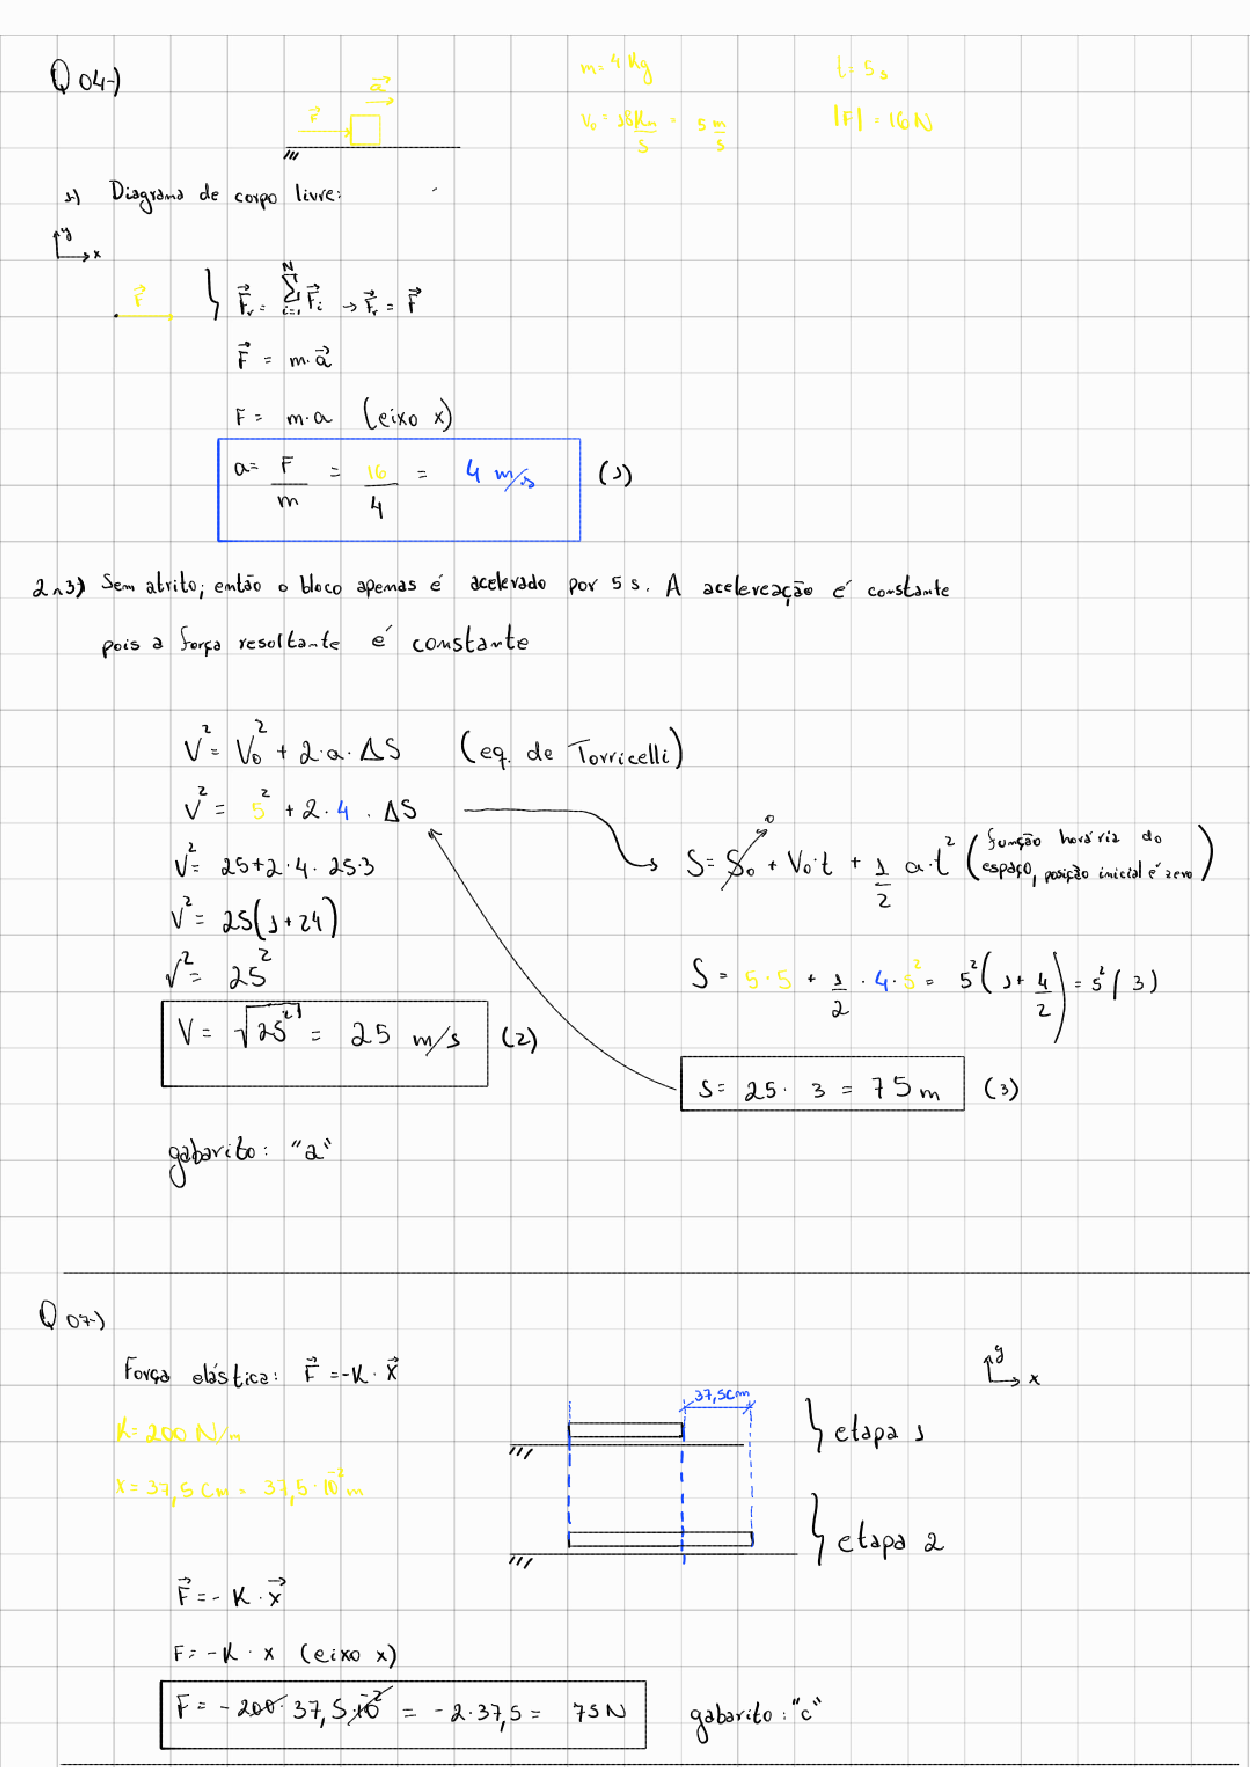
\includepdf[pages=1, scale=0.85, offset=0 -1.4cm,
  pagecommand=\tituloanexo]{resolucoes_dinamica.pdf}

\includepdf[pages=2-, scale=0.95,
  pagecommand={\thispagestyle{empty}}]{resolucoes_dinamica.pdf}

\end{document}
